\documentclass[a4paper,UTF8]{ctexart}

\usepackage{amsmath, amsthm, amssymb, amsfonts, hyperref, mathrsfs}%美国数学学会的包+?
\usepackage{geometry} %控制界面
\usepackage{bookmark}
\usepackage{fancyhdr} % header & footer
\usepackage{appendix} % 附录
\usepackage{tikz} %作图
\usepackage{graphicx} %插入图片的宏包
\usepackage{float} %设置图片浮动位置的宏包
\usepackage{subfigure} %插入多图时用子图显示的宏包
\usepackage{listings} %引用代码
\usepackage{physics,mathtools} %物理数学工具
\usepackage{comment}
\usepackage{framed}
\geometry{top=2.5cm,bottom=2.5cm,left=2.5cm,right=2.5cm} % 布局要求
\pagestyle{fancy} % fancy分格
\fancyhf{} % 清除所有页眉页脚
\renewcommand\headrulewidth{0.6pt}
\renewcommand\footrulewidth{0.6pt}
\lhead{何金铭 PB21020660$\mid$座位号:3}
\chead{氢氘光谱实验报告}
\rhead{\thepage}
\lfoot{2023.4.3}
\rfoot{USTC}
%\bibliographystyle{plain} % 引用样式
\everymath{\displaystyle} % display
%============================================================

\begin{document}

\begin{center}
    \textbf{\Large 氢氘光谱实验报告}
    \par \text{\large 何金铭 PB21020660}
\end{center}

\section{实验目的}

\begin{enumerate}
    \item 探究同位素的原子光谱是否有区别
    \item 了解光栅光谱仪的构造,并使用其测量光谱
    \item 通过光谱测量计算氢氘巴尔末线系前四条谱线的波长、里德伯常数$R_{H}$和氢
氘的质量比
\end{enumerate}

\section{实验原理}

\subsection{同位素与同位素位移}
在谱线上,同位素对应的谱线会发生移位,称同位素移位。移位大小与核质
量有关:核质量越轻,移位效应越大,因此氢具有最大的同位素移位。
\subsection{原子光谱规律}

主要利用氢氘原子巴尔末系的光谱线$H_{\alpha},H_{\beta},H_{\gamma},H_{\delta}$,来进行测量,有巴尔末公式:

\begin{equation}
    \tilde{\nu} = R_{H} (\frac{1}{2^2}-\frac{1}{n^2})
\end{equation}

通过对里德伯常数计算的修正,可以给出氘核里德伯常数的修正公式:

\begin{equation}
    R = \frac{R_{\infty}}{1+\frac{m_{e}}{M}}
\end{equation}

再利用一些简单的推导也可以导出一些计算公式:

\begin{equation}
    \frac{M_{D}}{M_{H}} = \frac{\frac{R_{D}}{R_{H}}}{1-(\frac{R_{D}}{R_{H}}-1)\frac{M_{H}}{m_{e}}}
\end{equation}

\begin{equation}
    \frac{M}{m} \approx \frac{\lambda}{2 \Delta \lambda}
\end{equation}

这些公式分别可以计算得氢氘核质量比和质子电子质量比,具体的推导于数据分析中展开。

\section{实验仪器}

氢氘光栅实验仪器(光源配有汞灯和氢氘灯)

\section{实验数据处理}

\subsection{原始实验数据}

\begin{table}[H]
    \centering
    \begin{tabular}{|c|c|c|c|c|c|}
    \hline
        汞灯谱线序号 & 1 & 2 & 3 & 4 & 5 \\ \hline
        $\lambda /nm$ & 365.16 & 365.64 & 366.44 & 404.82 & 407.78 \\ \hline
        汞灯谱线序号 & 6 & 7 & 8 & 9 &  \\ \hline
        $\lambda /nm$ & 435.88 & 546.02 & 577.10 & 579.08 &  \\ \hline
    \end{tabular}
    \caption{不同汞灯谱线的波长记录表}
\end{table}

\begin{table}[H]
    \centering
    \begin{tabular}{|c|c|c|c|c|}
    \hline
        能级n & 3 & 4 & 5 & 6 \\ \hline
        $\lambda_{H}/nm$ & 657.26 & 486.54 & 433.93 & 409.98 \\ \hline
        $\lambda_{D}/nm$ & 657.13 & 486.42 & 433.82 & 409.87 \\ \hline
    \end{tabular}
    \caption{巴尔末系不同能级的氢氘谱线波长记录表}
\end{table}

{\bfseries 注:在记录表二的时候发生了记录顺序的错误,这里已经给出了修正,具体的记录顺序错误可见原始数据上红笔解释。}

\subsection{汞灯标准谱线和测量谱线拟合方程和拟合数据图}

假设光谱的误差是线性的,设转换公式有形式$\lambda^{*} = a \lambda_{measure} + b$,记标准值为$\lambda_{0}$

为求出参数$a,b$,则可使用最小二乘法来估计:

\begin{equation}
    \min{\sum_{i}{(\lambda^{*}_{i} - \lambda_{0i})^2}} = \min{\sum_{i}{(a \lambda_{measure_{i}} + b - \lambda_{0i})^2}}
\end{equation}

在$\lambda_{measure}$-$\lambda_{0}$平面中画出各个点$(\lambda_{measure},\lambda_{0})_{i}$,并用最小二乘法拟合,得:

\begin{equation}
    \lambda^{*} = 1.0004515 \lambda_{measure} - 0.2853027
\end{equation}

\begin{figure}[H]
    \centering
    \begin{minipage}[b]{0.9\textwidth}
        \centering
        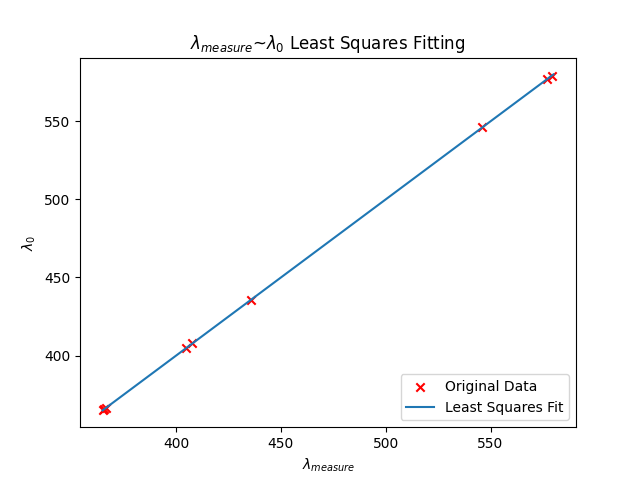
\includegraphics[width=0.8\textwidth]{./hr_fit.png}
        \caption{$\lambda_{measure}$-$\lambda_{0}$的最小二乘法拟合图}
    \end{minipage}
\end{figure}

\subsection{将氢氘谱线数据代入拟合方程后得到的近似校准后数据}

\begin{table}[H]
    \centering
    \begin{tabular}{|c|c|c|c|c|}
    \hline
        能级n & 3 & 4 & 5 & 6 \\ \hline
        $\lambda_{H}/nm$ & 657.27 & 486.47 & 433.84 & 409.88 \\ \hline
        $\lambda_{D}/nm$ & 657.14 & 486.35 & 433.73 & 409.77 \\ \hline
    \end{tabular}
    \caption{近似校准后巴尔末系不同能级的氢氘谱线波长记录表}
\end{table}

\subsection{计算氢氘谱线的里德伯常数、氢氘核质量比和质子电子质量比}

\subsubsection{氢氘谱线里德伯常数的计算}

可以利用下式进行计算:

\begin{equation}
    \tilde{\nu} = R_{H}(\frac{1}{2^2}-\frac{1}{n^2})
\end{equation}

\begin{equation}
    \tilde{\nu} = R_{D}(\frac{1}{2^2}-\frac{1}{n^2})
\end{equation}

\begin{table}[H]
    \centering
    \begin{tabular}{|c|c|c|c|c|}
    \hline
        能级n & 3 & 4 & 5 & 6 \\ \hline
        $R_{H}/10^7(m)^{-1}$ & 1.09544 & 1.09633 & 1.09762 & 1.09788 \\ \hline
        $R_{D}/10^7(m)^{-1}$ & 1.09566 & 1.0966 & 1.0979 & 1.09818 \\ \hline
    \end{tabular}
    \caption{利用不同能级计算得氢氘里德伯常数表}
\end{table}

氢氘里德伯常数的标准值为:氢的里德伯常数$R_{H} = 1.0967758 \times 10^7m^{-1}$,氘的里德伯常数$R_{D} = 1.0971 \times 10^{-7} m^{-1}$

对各组的测量值取平均值得:$R_{H}= 1.09682 \times 10^7 m^{-1},R_{D} = 1.09709 \times 10^7 m^{-1}$。取平均值的理由会于误差分析中提及。

\subsubsection{氢氘核质量比的计算}

由于

\begin{equation}
    R_{H} = \frac{R_{\infty}}{1+\frac{m_{e}}{M_{H}}}
\end{equation}

\begin{equation}
    R_{D} = \frac{R_{\infty}}{1+\frac{m_{e}}{M_{D}}}
\end{equation}

由此得出:

\begin{equation}
    \frac{M_{D}}{M_{H}} = \frac{\frac{R_{D}}{R_{H}}}{1-(\frac{R_{D}}{R_{H}}-1)\frac{M_{H}}{m_{e}}}
\end{equation}

代入$\frac{R_D}{R_H} = \frac{1.09709}{1.09682} =1.00025,\frac{M_H}{m_e} = 1836.1527$得:

\begin{equation}
    \frac{M_D}{M_H} = \frac{1.00025}{1-(1.00025-1)\cdot 1836.1527} = 1.82526
\end{equation}

\subsubsection{质子电子质量比的计算}

\begin{equation}
    \Delta \lambda = \lambda_{H} - \lambda_{D} = \frac{\frac{1}{R_{H}}-\frac{1}{R_{D}}}{\frac{1}{2^2}-\frac{1}{n^2}} \approx \frac{\frac{M+m}{M}-\frac{2M+m}{2M}}{\frac{1}{\lambda}} = \frac{m}{2M} \lambda
\end{equation}

得:

\begin{equation}
    \frac{M}{m} \approx \frac{\lambda}{2 \Delta \lambda}
\end{equation}

代入$\lambda = 409.88nm, \Delta \lambda = 409.88-408.77 = 0.11nm$得:

\begin{equation}
    \frac{M}{m} = \frac{409.88nm}{2\times 0.11nm} = 1863.09
\end{equation}

\begin{table}[H]
    \centering
    \begin{tabular}{|c|c|c|c|c|}
    \hline
        能级n & 3 & 4 & 5 & 6 \\ \hline
        $\frac{M_{H}}{m_{e}}$ & 2527.96 & 2026.96 & 1972.0 & 1863.09 \\ \hline
    \end{tabular}
    \caption{利用不同能级计算得质子电子质量比表}
\end{table}

发现利用不同能级的数据计算得的结果不同,代入能级为6的数据时,计算的结果与理论值最为接近。

\section{实验总结和误差分析}

\subsection{误差分析}

\subsubsection{里德伯常数的误差分析}

对于氢氘光谱,利用不同能级算得的里德伯常数不同,而且发现能级为3时,测得的$R$最小,随着能级的增加,测得的里德伯常数也越来越大。

但发现分别对$R_{H},R_{D}$取平均值,得到的值则与理论值极为接近,相对误差小于$0.1\%$。

不同能级间造成的差异,是由不同能级测得的光谱波长存在差异导致的。分析得,低能级测得的波长偏大;高能级测得的波长偏小。可能的原因是:转换公式
    $\lambda^{*} = 1.0004515 \lambda_{measure} - 0.2853027$不够准确。
是转换方程的拟合斜率值过大导致的。可能的原因有:

\begin{enumerate}
    \item 首先其转换公式只是平方范数意义下的最小误差,也是不准确的。可以尝试一些其它的误差逼近函数。
    \item 其次,我们做出的假设是:光谱的误差是线性的。所以采取了上述做法。然后实际上误差也可能是未知形式的非线性误差,需要做更加细致的实验进行分析,或者尝试一些其它的误差形式。
    \item 最后,也可能会有一些实验中其它的问题。比如说没有考虑空气折射率对实验的影响;汞灯做实验的时候没有完成预热;测量汞灯光谱时采用的扫描间隔为0.02nm,不是很精确,但这一点只有比较小的影响。
\end{enumerate}

设准确的转换方程为:

\begin{equation}
    \lambda ^* = a_0 \lambda_{measure} + b_0
\end{equation}

所以我们的误差公式可以改写为形式:

\begin{equation}
    \lambda^* = (a_0 - (a_0 - a_{fit})) \lambda_{measure} + (b_0 - (b_0 - b_{fit})) = (a_0 - \Delta a_0) \lambda_{measure} + (b_0 - \Delta b_0) 
\end{equation}

式中,$\Delta a_0$代表拟合转换方程的斜率误差,$\Delta b_0$代表拟合转换方程的截距误差。

取平均数近似的话,可以消除一部分由于线性误差带来的影响:因为波长在转换方程的左右分布较为均匀,所以左右的差距可以消除一部分,可以做到稍微精确一些。

若要分析的更精确,可以考虑使用最小二乘法使得左右由斜率带来的误差最小,具体的数学形式就不在这里展开。

\subsubsection{氢氘核质量比的误差分析}

计算得$\frac{M_{D}}{M_{H}} = 1.82526$,与理论值$2$较为接近,其中主要造成误差的是$\frac{R_D}{R_H}$的精确度。
当$\frac{R_D}{R_H}$的比值发生一点微小的变化时,就会对结果产生很大的影响。

而$\frac{R_D}{R_H}$主要是由$R_{H},R_{D}$的测量决定的,而$R_{H},R_{D}$的误差分析已经在前面分析过了。

\subsubsection{质子电子质量比的误差分析}

发现利用不同能级计算结果的时候,结果会发生很大的不同。当利用能级6计算的时候,与结果1836.15最为接近;而当能级数降低的时候,计算的结果也越来越大,越偏离理论值。
这说明低能级的波长测量值$\lambda$偏大或者同位素的波长位移$\Delta \lambda$偏小。

可能的原因有:

\begin{enumerate}
    \item 继续上面的讨论,若转换方程的斜率拟合值偏大,则会使得波长长的能级(能级小的能级)产生很大的误差,可能的原因已经于上文给出。
    \item 分析$\Delta \lambda$偏小的原因:在测量的时候,通过0.01nm的步长进行扫描,然后由于点是离散的,实际的最大值可能在测量峰值的左右两格的间隔之内。
    由于同位素的波长位移$\Delta \lambda_{true}$很小,约为0.11nm,而由于步长带来的测量误差有平均0.01nm,这个误差实际上是很大的。
    \item 其它的原因有:比如说没有考虑空气折射率对实验的影响;氢氘灯做实验的时候没有完成预热;狭缝的宽度对实验现象的影响等。
\end{enumerate}

\subsection{实验总结}

\begin{enumerate}
    \item 可以明显的观察到氢氘同位素光谱中的谱线位移。
    \item 利用光栅光谱仪测量了氢氘光谱巴尔末系的波长值,测得的氢的里德伯常数为$R_{H} = 1.09682 \times 10^7 m^{-1}$,氘的里德伯常数为$R_{D}= 1.09709 \times 10^7 m^{-1}$
    \item 测得的氘氢核质量比为$\frac{M_{D}}{M_{H}} = 1.82526$
    \item 测得的质子电子质量比为$\frac{M_{H}}{m_{e}} = 1863.09$
    \item 实验中也存在很多误差,于上文的误差分析中有详细说明,这里不重复说明。
\end{enumerate}

\section{思考题}

\subsection{在计算$R_{H}$、$R_{D}$时,应该以真空中的波长代入公式计算,但实验中的测量是在空
气中进行的。若空气的折射率为 $n=1.00029$,请推导波长修正公式,并将修正后的 $R_{H}$、$R_{D}$ 值与公认值比较。}。

真空中的波长$\lambda_{vacuum}$与空气中波长$\lambda_{air}$有关系:

\begin{equation}
    \lambda_{vacuum} = n \lambda_{air}
\end{equation}

所以真实的里德伯常数应修正为:

\begin{equation}
    R_{H}' = \frac{R_{H}}{n} = 1.0965 \times 10^7 m^{-1}
\end{equation}

\begin{equation}
    R_{D}' = \frac{R_{D}}{n} = 1.09677 \times 10^7 m^{-1}
\end{equation}

发现修正后的$R_{H},R_{D}$均偏小了,可能存在的误差于上文误差分析中有提及。

\subsection{本实验中测量汞灯光谱目的是什么?请问若要使用其他光源或者方法代替测
量汞灯光谱,给出方案。}

为了校准光栅光谱仪,借助于波长已知的线光谱光源(于此处是汞灯光谱)来对单色仪测量的波长进行标定,校正在使用过程中产生的波长位置误差,来保证测量的波长位置的准确性。

可以利用其它的光源来校准汞灯光谱,比如可以利用氦氖激光发生器或低压钠灯来进行校准。

具体方案与本实验中的类似:

\begin{enumerate}
    \item 先调试好仪器设备,搭好光路。
    \item 选择一个合适的入射狭缝宽度,并且选取一个合适的负高压,测量时须找出合适的负高压值,
    并利用采集程序设定合理的测量范围获取光谱线完全分离开的光谱曲线
\end{enumerate}

\subsection{若想要测量其他元素同位素光谱,对仪器有什么要求?为什么?}

\begin{enumerate}
    \item 要求仪器中光栅的色分辨本领要高。由于同位素效应带来的光谱位移极小,若分辨本领低,则无法分辨出光谱中的两个峰。
    \item 不仅如此,还要求步进电机每一步可以转动的足够的小,以便可以转动到合适的角度。
\end{enumerate}



\end{document}